%% LyX 2.4.0~RC3 created this file.  For more info, see https://www.lyx.org/.
%% Do not edit unless you really know what you are doing.
\documentclass[french]{beamer}
\usepackage[T1]{fontenc}
\usepackage[utf8]{inputenc}
\setcounter{secnumdepth}{3}
\setcounter{tocdepth}{3}
\usepackage{url}
\usepackage{amstext}
\usepackage{amssymb}
\usepackage{graphicx}
% import listings package
\usepackage{minted}

\synctex=1
\makeatletter

%%%%%%%%%%%%%%%%%%%%%%%%%%%%%% LyX specific LaTeX commands.
%% Because html converters don't know tabularnewline
\providecommand{\tabularnewline}{\\}

%%%%%%%%%%%%%%%%%%%%%%%%%%%%%% Textclass specific LaTeX commands.
% this default might be overridden by plain title style
\newcommand\makebeamertitle{\frame{\maketitle}}%
% (ERT) argument for the TOC
\AtBeginDocument{%
  \let\origtableofcontents=\tableofcontents
  \def\tableofcontents{\@ifnextchar[{\origtableofcontents}{\gobbletableofcontents}}
  \def\gobbletableofcontents#1{\origtableofcontents}
}

%%%%%%%%%%%%%%%%%%%%%%%%%%%%%% User specified LaTeX commands.

\AtBeginSection[]{
  \begin{frame}
  \vfill
  \centering
  \begin{beamercolorbox}[sep=8pt,center,shadow=true,rounded=true]{title}
    \usebeamerfont{title}\insertsectionhead\par%
  \end{beamercolorbox}
  \vfill
  \end{frame}
}

\setbeamertemplate{navigation symbols}{}

\addtobeamertemplate{navigation symbols}{}{%
    \usebeamerfont{footline}%
    \usebeamercolor[fg]{footline}%
    \hspace{1em}%
    \insertframenumber/\inserttotalframenumber
}



\makeatother


\begin{document}
\title{LLM fine-tuning for time series annotation}
\author{Philippe Helluy}
\institute{IRMA, Université de Strasbourg, Inria Tonus}
\makebeamertitle
\begin{frame}{Outlines}

\tableofcontents{}
\end{frame}
%

\section{How it works (roughly...)}
\begin{frame}{Very brief history}
\begin{itemize}
\item Artificial neural networks have existed for a \textbf{long time}
(\cite{rosenblatt1958perceptron}, late 1950s). 
\item Ups and downs, then \textbf{Yann LeCun} (\cite{lecun1989backpropagation},
handwriting recognition, 1989).
\item \emph{Attention is all you need} \cite{vaswani2017attention}, invention
of \textbf{transformers} at Google. 
\item Without huge \textbf{computing power}, it would not work.
\end{itemize}
\end{frame}
%
\begin{frame}{\emph{Completion is all you need}}
\begin{itemize}
\item Principle: we are given the beginning of a text. The task is to predict the next word.
Example: \textquotedbl the cat eats the ...\textquotedbl{} (we must guess \textquotedbl mouse\textquotedbl).
\item Words (or \emph{tokens}):\\
\begin{tabular}{|c|c|c|c|c|c|}
\hline 
$t_{1}$ & $t_{2}$ & $t_{3}$ & $t_{4}$ & $t_{5}$ & $t_{6}=t_{m}$\tabularnewline
\hline 
\hline 
. & cat & the & eats & tomcat & mouse\tabularnewline
\hline 
\end{tabular}
\item Corpus: \textquotedbl the cat eats the mouse.\textquotedbl , \textquotedbl the
tomcat eats the mouse.\textquotedbl , \textquotedbl ..the cat eats.\textquotedbl ,
\textquotedbl ..the mouse eats.\textquotedbl , \textquotedbl ..the
tomcat eats.\textquotedbl , \emph{etc.}
\item Remark: all sentences have $\ell=6$ words (we pad with the filler word \textquotedbl .\textquotedbl).
\end{itemize}
\end{frame}
%
\begin{frame}{Digitization}
\begin{itemize}
\item Encoding: to each word (or \emph{token}) we associate a vector of $m=6$
dimensions{\footnotesize
\[
\text{"."}=\left[\begin{array}{c}
1\\
0\\
0\\
0\\
0\\
0
\end{array}\right],\quad\text{"cat"}=\left[\begin{array}{c}
0\\
1\\
0\\
0\\
0\\
0
\end{array}\right],\quad\text{"the"}=\left[\begin{array}{c}
0\\
0\\
1\\
0\\
0\\
0
\end{array}\right],\quad\text{\emph{etc.}}
\]
}{\footnotesize\par}
\item Embedding into a lower-dimensional space of size $p$ (to account for synonyms, among other things). For example
$p=5$. The embedding $E_{w_{0}}$ is a function from $\mathbb{R}^{m}$
to $\mathbb{R}^{p}$.
\item Each token $t_{i}$ is represented by a vector $v_{i}$. The embedding
parameters $w_{0}$ are unknown. 
\[
v_{i}=E_{w_{0}}(t_{i}).
\]
\end{itemize}
\end{frame}
%
\begin{frame}{Encoder}
\begin{itemize}
\item A sentence is thus represented by a \textquotedbl tensor\textquotedbl{}
of $\ell$ numerical vectors stacked together:
\[
r_{0}=v_{i_{1}}v_{i_{2}}\ldots v_{i_{\ell}}
\]
It is therefore an object in a space of dimension $N=\ell\times p=30$.
\item The sentence goes through $k$ layers of transformers $T_{w_{i}}$,
which are mappings from $\mathbb{R}^{N}$ to $\mathbb{R}^{N}$
with unknown parameter vectors $w_{i}$
\[
r_{i}=T_{w_{i}}(r_{i-1}),\quad i=1\ldots k.
\]
\item The deeper we go into the layers, the more abstract 
the representation $r_{i}$ of the initial sentence becomes. The vector
$r_{k}$ ("latent state") contains the information extracted by the network from the initial
sentence $r_{0}.$
\end{itemize}
\end{frame}

%
\begin{frame}{Decoder}

Finally, the decoder allows us to predict a probability vector
$p$ in $\mathbb{R}^{m}$: $p_{i}$ is the probability that the next word
is $m_{i}$.
\[
p=D_{w_{k+1}}(r_{k}).
\]
In summary (more details in \cite{tunstall2022natural,vigon2023}):
\begin{center}
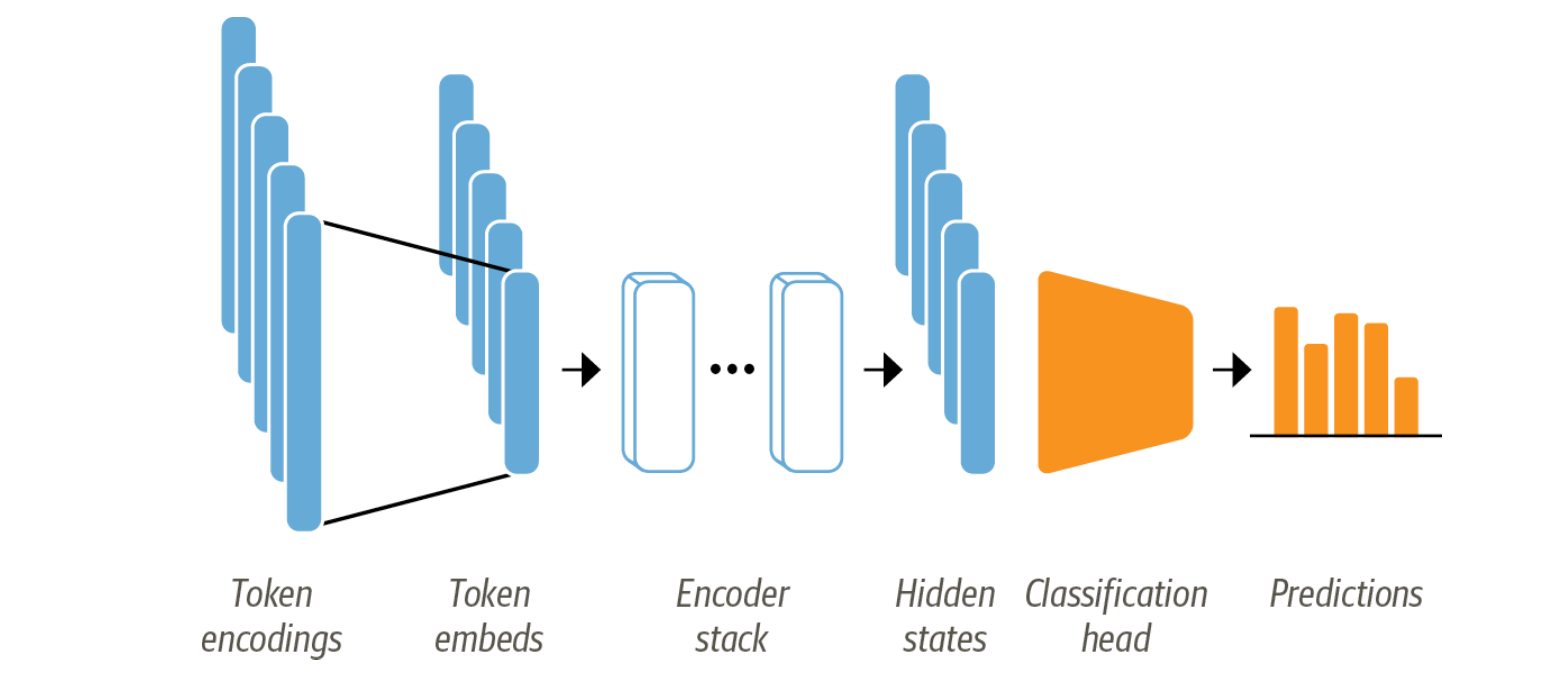
\includegraphics[width=0.9\textwidth]{../../IMPORTANT/Recherche/PyTorch/encode-decode}
\par\end{center}

\end{frame}
%
\begin{frame}{Training}
\begin{itemize}
\item Choosing the form of the functions $E_{w_{0}}$, $T_{w_{i}}$, $D_{w_{k+1}}$:
a trade-off between cost, efficiency, and simplicity. For now, it is
as much an art as it is a science.
\item Historically, several possible architectures: CNN, RNN, LSTM, transformers.
Evolution is strongly linked to available computing power.
\item The parameter vector $w$, of size $s$, is \textbf{unknown}.
\item Training consists in optimizing these parameters so that the model
best reproduces the sentences from the corpus.
\item This is the most difficult part of the computation: it requires a supercomputer,
specialized processors, and costs millions of euros.
\item Orders of magnitude for GPT-3: $\ell=2000$, $m=50000$, $p=20000$,
$s=170$ billion...
\end{itemize}
\end{frame}
%
\begin{frame}{Inference}
\begin{itemize}
\item Once the parameters $w$ are computed, inference is fast.
\item A network can be retrained for a specific task at a reduced cost
(\emph{fine tuning}). For example, Copilot and ChatGPT are specialized
versions of GPT-3.
\item The \textit{pre-prompt} is essential to obtain high-quality results.
\item For computational cost reasons, \textbf{ChatGPT does not learn in
real time}. Its short-term memory is therefore limited to a few
thousand words.
\end{itemize}
\end{frame}
%
\begin{frame}{Example with PyTorch}
\begin{itemize}
\item PyTorch is a free software library developed by Huggingface
to manipulate neural networks.
\item Minimal usage example.
\end{itemize}
\end{frame}

\section{Fine tuning of Qwen LLM for time series annotation}
\begin{frame}[fragile]{Objectives}

\begin{itemize}
\item Teach a small LLM (Qwen2.5 0.5 billions parameters) to describe a
time series
\item Example of prompt:\\
\begin{minted}[fontsize=\tiny]{markdown}
Describe the time series in three sentences.
First sentence: describe trend (increasing/decreasing/flat).
Second sentence: noise intensity (low/medium/high).
Third sentence: approximate localisation of global maximum (beginning/middle/end)
and global minimum (beginning/middle/end).
Put the description in a JSON format with the following pattern
<json>{ "trend": <sentence1>,
"noise": <sentence2>,
"extrema": <sentence3> }
</json>
Series: [02, 01, 00, 03, ... ]
\end{minted}
\item Tokenization is essential: the values in the series are scaled to the range 00..99.
\end{itemize}
\end{frame}

\begin{frame}[fragile]{Necessity of training}

\begin{itemize}
\item Small LLM fails to answer properly. It generates total garbage.
\item Example of output:\\
\begin{minted}[fontsize=\tiny]{markdown}
series name: \"series\"
time interval: 1 day
``` To provide a detailed analysis of the given time series data, I will break it down into its components:
### Time Series Description:
The provided time series consists of daily values for several variables over a period of one year (assuming 365 days).
### Trend Analysis:
- **Increase**: The values increase steadily from 01 to 04, then decrease again.
- **Decrease**: The values decrease from 04 onwards
...
\end{minted}
\item Let's try to improve this with supervised fine tuning
\end{itemize}
\end{frame}

\begin{frame}[fragile]{Practical methodology}

\begin{itemize}
\item Generate a dataset of correct examples with a large LLM (Mistral, ChatGPT, etc.)
\item Apply a supervised fine tuning (SFT) procedure on a small LLM from this dataset.
\item In order to reduce the cost we adopt a LoRA approach. \footnote{The LoRA (Low-Rank Adaptation) approach in supervised fine-tuning (SFT) freezes the original model weights and injects small trainable low-rank matrices into certain layers (typically linear projections in attention/FFN). This drastically reduces the number of parameters that need updating, making fine-tuning large models much more memory- and compute-efficient while still achieving strong adaptation.}
\item Now go to \url{https://github.com/phelluy/DLAA_2025} and follow the README file.
\end{itemize}
\end{frame}
%
\begin{frame}[allowframebreaks]{Bibliographie}

\tiny\bibliographystyle{apalike-fr}
\nocite{*}
\bibliography{copilot}

\end{frame}

\end{document}
